% vim:encoding=utf8 ft=tex sts=2 sw=2 et:

\documentclass{classrep}
\usepackage[utf8x]{inputenc}
\usepackage[a4paper, left=2.0cm, right=2.0cm, top=1.5cm, bottom=2.0cm, headsep=0.5cm, headheight=15pt]{geometry}
\usepackage{amsmath, amsthm, amssymb, amsfonts}
\usepackage{graphicx}
\usepackage{float}
\usepackage{listings}
\lstdefinelanguage{VHDL}{
	morekeywords={
		library,use,all,entity,is,port,in,out,end,architecture,of,
		begin,and,LIBRARY,USE,ALL,ENTITY,IS,PORT,IN,OUT,END,ARCHITECTURE,OF,BEGIN,AND
	},
	morecomment=[l]--
}

\usepackage{xcolor}
\colorlet{keyword}{blue!100!black!80}
\colorlet{comment}{green!90!black!90}
\lstdefinestyle{vhdl}{
	language     = VHDL,
	basicstyle   = \ttfamily,
	keywordstyle = \color{keyword}\bfseries,
	commentstyle = \color{comment}
}
\lstset{language=VHDL,style=vhdl}

\studycycle{Elektronika i Telekomunikacja, studia dzienne, mgr II st.}
\coursesemester{I}

\coursename{Programowalne układy cyfrowe}
\courseyear{2014/2015}

\courseteacher{mgr. Tomaszewski Grzegorz}
\coursegroup{poniedziałek, 14:00}

\author{
  \studentinfo{Witold Olechowski}{127517} \and
  \studentinfo{Tomasz Marecik}{127374}
}

\title{Zadanie 2: Realizacja prostych funkcji logicznych w strukturze FPGA}

\usepackage{hyperref} % musi być na końcu
\hypersetup{pdfborder={0 0 0 0}}
\begin{document}
\maketitle

\section{Minimalizacja funkcji logicznych}
Zrealizować i zminimalizować funkcje logiczną 
$F(DCBA)= \varSigma \{0,1,2,5,8,9,10,13,15,(3)\} \label{fdcba}$

\begin{figure}[H]
	\centering
	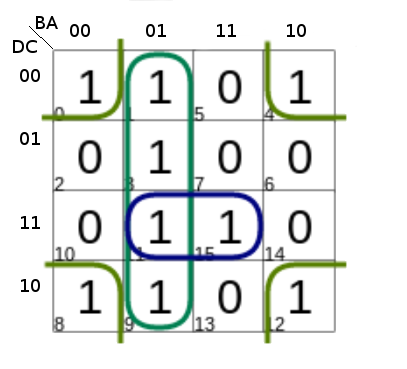
\includegraphics[width=0.4\linewidth]{kar}
	\caption{Minimalizacja funkcji przy pomocy siatki Karnaugha}
	\label{fig:kar}
\end{figure}

$F(DCBA)=\bar{B} A \cup DCA \cup \bar{A} \bar{C}$

\begin{figure}
	\centering
	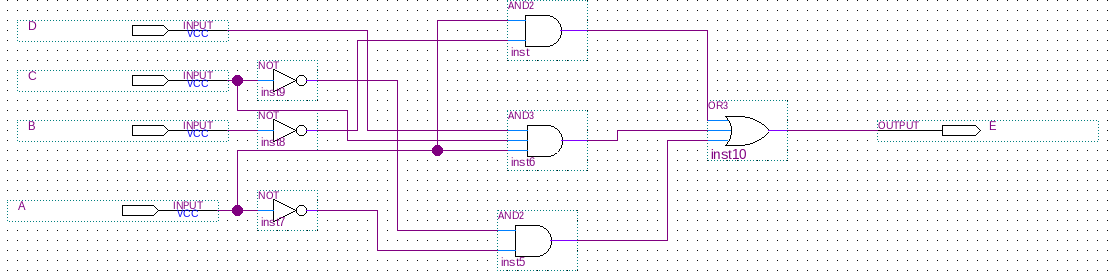
\includegraphics[width=1.0\linewidth]{block}
	\caption{Realizacja funkcji na bramkach logicznych}
	\label{fig:block}
\end{figure}

\section{Realizacja funkcji$_{\ref{fdcba}}$ w środowisku Quarus II}
Na rysunku \ref{fig:block} przedstawiono realizację jako blok funkcyjny, ponizej znajduje się jej analogia w języku VHDL.

\lstinputlisting{block1.vhdl}

\subsection{Symulacja}
 \begin{figure}[H]
\centering
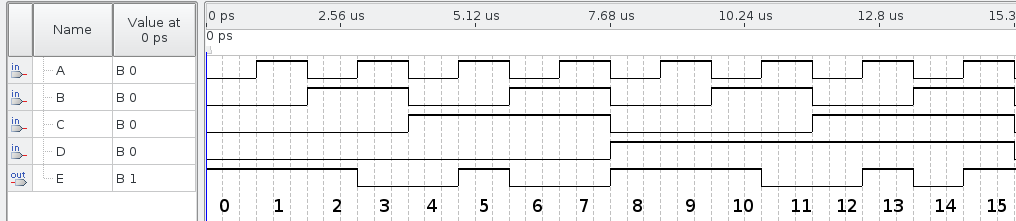
\includegraphics[width=1.0\linewidth]{symf}
\caption{Symulacja działania układu}
\label{fig:symf}
\end{figure}

\section{Blok funkcyjny realizujacy sume i iloczyn logiczny}

\begin{figure}[H]
\centering
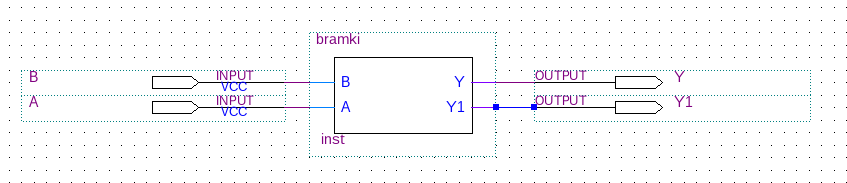
\includegraphics[width=0.8\linewidth]{blokvramek}
\caption{Blok funkcyjny gdzie: Y - realizuje iloczyn, Y1 - sumę }
\label{fig:blokvramek}
\end{figure}

 \vskip 2\baselineskip

\lstinputlisting{bramki.vhd}
\subsection{Symulacja}
\begin{figure}[H]
\centering
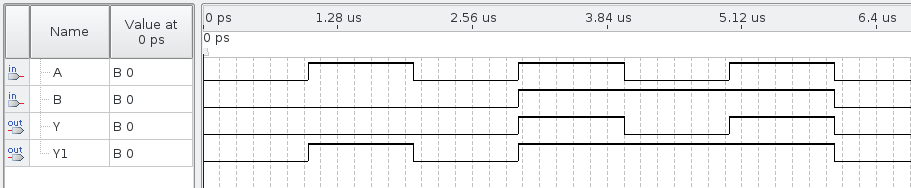
\includegraphics[width=1.0\linewidth]{bramki}
\caption{Symulacja działania układu}
\label{fig:bramki}
\end{figure}

\section{Wnioski}
\begin{itemize}
	\item szybsze projektowanie logiki w VHDL niż BFD
\end{itemize}

\begin{thebibliography}{0}
  \bibitem{l2short} John Wiley and Sons Publishers.
    \textsl{Digital Design,} University of California, Riverside, 2007
\end{thebibliography}
\end{document}
